\documentclass[9pt,a4paper]{extarticle}

% ── Paquetes ──
\usepackage[utf8]{inputenc}
\usepackage[T1]{fontenc}
\usepackage[defaultfam,tabular,lining]{montserrat}
\usepackage[spanish]{babel}
\usepackage{geometry}
\usepackage{graphicx}
\usepackage{array}
\usepackage{booktabs}
\usepackage{longtable}
\usepackage{enumitem}
\usepackage{xcolor}
\usepackage{titlesec}
\usepackage{hyperref}
\usepackage{fancyhdr}
\usepackage{tabularx}
\usepackage{multirow}
\usepackage{parskip}
\usepackage{float}
\usepackage{colortbl}

% ── Ruta de imagenes ──
\graphicspath{{diagramas-excalidraw/imagenes/}}

% ── Geometria ──
\geometry{left=2.5cm, right=2.5cm, top=3cm, bottom=2.5cm, headheight=35pt}

% ── Colores ──
\definecolor{cruzroja}{RGB}{200, 16, 46}
\definecolor{grisoscuro}{RGB}{64, 64, 64}
\definecolor{grisclaro}{RGB}{240, 240, 240}
\definecolor{azullink}{RGB}{0, 90, 156}
\definecolor{azuloscuro}{RGB}{0, 51, 102}
\definecolor{azulmedio}{RGB}{0, 90, 156}
\definecolor{azulclaro}{RGB}{41, 128, 185}
\definecolor{verdeclaro}{RGB}{220, 245, 220}
\definecolor{amarilloclaro}{RGB}{255, 250, 220}
\definecolor{rojoclaro}{RGB}{255, 230, 230}

% ── Estilos de titulos ──
\titleformat{\section}{\Large\bfseries\color{azuloscuro}}{}{0em}{}[\vspace{-0.5em}{\color{azuloscuro}\rule{\textwidth}{0.5pt}}]
\titleformat{\subsection}{\large\bfseries\color{azulmedio}}{}{0em}{}
\titleformat{\subsubsection}{\normalsize\bfseries\color{azulclaro}}{}{0em}{}

% ── Hyperlinks ──
\hypersetup{
    colorlinks=true,
    linkcolor=azuloscuro,
    urlcolor=azulmedio,
    citecolor=azuloscuro
}

% ── Encabezado y pie ──
\pagestyle{fancy}
\fancyhf{}
\fancyhead[L]{
\includegraphics[height=1.1cm]{logo-full.pdf}}
\fancyhead[R]{\small\color{grisoscuro}Sistema de Gesti\'{o}n de Programaciones}
\fancyfoot[C]{\small\color{grisoscuro}\thepage}
\renewcommand{\headrulewidth}{0.4pt}
\renewcommand{\footrulewidth}{0pt}

% ── Metadatos ──
\title{
    \vspace{-1cm}
    {\color{azuloscuro}\rule{\textwidth}{2pt}}\\[0.8cm]
    
\includegraphics[height=3cm]{logo-full.pdf}\\[0.8cm]
    {\Huge\bfseries\color{azuloscuro} Sistema de Gesti\'{o}n de\\[0.3cm] Programaciones}\\[0.5cm]
    {\Large\color{azulmedio} Documento de Validaci\'{o}n Funcional}\\[0.3cm]
    {\large\color{azulclaro} Para revisi\'{o}n de involucrados}\\[0.5cm]
    {\color{azuloscuro}\rule{\textwidth}{2pt}}
}
\author{
    \textbf{Cruz Roja Colombiana Seccional Antioquia}\\
    \ Transformaci\'{o}n Digital
}
\date{Febrero 2026 -- Versi\'{o}n 1.0}

\begin{document}

\maketitle
\thispagestyle{empty}
\newpage

\tableofcontents
\newpage

% ══════════════════════════════════════════════════════════════
\section{Prop\'{o}sito de este Documento}
% ══════════════════════════════════════════════════════════════

Este documento presenta las funcionalidades, reglas y flujos de trabajo del \textbf{Sistema de Gesti\'{o}n de Programaciones} para que los equipos involucrados puedan revisar y validar que el sistema refleja correctamente la operaci\'{o}n real.

\subsection{?`Qu\'{e} necesitamos de usted?}

Al revisar este documento, por favor confirme o corrija:

\begin{itemize}[leftmargin=2em]
    \item ?`Los \textbf{flujos de trabajo} descritos corresponden a c\'{o}mo operan hoy (o c\'{o}mo deber\'{i}an operar)?
    \item ?`Las \textbf{reglas de negocio} (l\'{i}mites de horas, domingos, pernoctas, municipios) son correctas?
    \item ?`Los \textbf{roles y permisos} reflejan qui\'{e}n debe ver y hacer qu\'{e}?
    \item ?`Los \textbf{datos de campañas} (tamaños, modalidades, estados) est\'{a}n completos?
    \item ?`Falta alg\'{u}n caso, excepci\'{o}n o situaci\'{o}n que no est\'{e} contemplada?
\end{itemize}


% ══════════════════════════════════════════════════════════════
\section{Contexto y Justificaci\'{o}n}
% ══════════════════════════════════════════════════════════════

\subsection{Situaci\'{o}n Actual}

La Cruz Roja Colombiana Seccional Antioquia gestiona m\'{u}ltiples operaciones que requieren la programaci\'{o}n de personal especializado. La primera implementaci\'{o}n se enfoca en el \'{a}rea de \textbf{Banco de Sangre}, donde se programa personal de diferentes perfiles (bacteri\'{o}logos, m\'{e}dicos, t\'{e}cnicos operativos y t\'{e}cnicos administrativos) para \textbf{turnos en sede principal} (en diferentes \'{a}reas, incluyendo punto fijo) y para \textbf{campañas extramurales} de donaci\'{o}n de sangre. \textbf{No todo el personal participa en ambos modelos:} algunos perfiles trabajan exclusivamente en sede (turnos en diferentes \'{a}reas y punto fijo), mientras que otros rotan entre sede y campañas extramurales.

La programaci\'{o}n actual se realiza mediante \textbf{hojas de c\'{a}lculo (Excel / Google Sheets)}, lo cual genera los siguientes problemas:

\begin{itemize}[leftmargin=2em]
    \item No existe visibilidad en tiempo real de las horas extras acumuladas por cada empleado.
    \item El equipo comercial no tiene forma de consultar la disponibilidad real del personal antes de gestionar campañas.
    \item No se validan autom\'{a}ticamente conflictos de horario, l\'{i}mites legales, ni restricciones mensuales (domingos, pernoctas).
    \item Las campañas pueden programarse con muy poca anticipaci\'{o}n o cancelarse el d\'{i}a anterior, sin un flujo formal de gesti\'{o}n.
    \item No hay trazabilidad de cambios ni hist\'{o}rico de asignaciones.
    \item La reducci\'{o}n progresiva de la jornada laboral en Colombia dificulta el cumplimiento de metas con los mismos recursos.
    \item El equipo comercial registra campañas en su CRM y las exporta a Excel; no hay integraci\'{o}n directa con Banco de Sangre.
    \item Los datos de donantes y c\'{o}digos de lugar provienen de Hexabank sin conexi\'{o}n automatizada.
\end{itemize}

\subsection{Visi\'{o}n del Sistema}

Se requiere un \textbf{sistema web} que automatice la gesti\'{o}n de programaciones, valide reglas laborales y brinde visibilidad a todos los roles involucrados.

El sistema se diseña como una \textbf{plataforma organizacional}: si bien la primera implementaci\'{o}n cubre la necesidad del banco de sangre, en el futuro puede extenderse a otras \'{a}reas como servicios de salud, Gesti\'{o}n del Riesgo, El Instituto y Log\'{i}stica.

% ══════════════════════════════════════════════════════════════
\section{Alcance de la Primera Implementaci\'{o}n}
% ══════════════════════════════════════════════════════════════

\begin{itemize}[leftmargin=2em]
    \item \textbf{Perfiles de personal:} Bacteri\'{o}logos, M\'{e}dicos, T\'{e}cnicos Operativos, T\'{e}cnicos Administrativos, personal Comercial y personal de Log\'{i}stica.
    \item \textbf{Dos flujos de programaci\'{o}n:}
    \begin{enumerate}
        \item \textbf{Turnos en sede principal} (jornada laboral regular, incluyendo diferentes \'{a}reas y punto fijo).
        \item \textbf{Campañas extramurales} (donaci\'{o}n de sangre fuera de sede).
    \end{enumerate}
    \item \textbf{Pool de personal:} No todo el personal participa en ambos modelos. Algunos perfiles trabajan exclusivamente en sede, mientras que otros rotan entre sede y campañas. Las horas de ambos flujos se suman para el c\'{o}mputo semanal.
    \item \textbf{\'{A}reas involucradas:} Banco de Sangre, Comercial, Log\'{i}stica.
    \item \textbf{Personal programado:} El sistema gestiona la programaci\'{o}n de \textbf{todo el personal} involucrado en la operaci\'{o}n, incluyendo personal operativo, comercial y de log\'{i}stica.
    \item \textbf{Usuarios estimados:} 30 a 100 usuarios.
    \item \textbf{Volumen:} +50 campañas por mes + turnos semanales en sede.
    \item \textbf{Integraciones:} CRM comercial (v\'{i}a Excel), Hexabank (c\'{o}digos de lugar y donantes).
\end{itemize}

% ══════════════════════════════════════════════════════════════
\section{Gesti\'{o}n de Campañas}
% ══════════════════════════════════════════════════════════════

\subsection{Tamaños de Campaña (Mix)}

Las campañas tienen cuatro tamaños predefinidos que determinan la composici\'{o}n del equipo:

\begin{table}[h!]
\centering
\begin{tabular}{|c|c|c|c|}
\hline
\textbf{Tamaño} & \textbf{Bacteri\'{o}logos} & \textbf{T\'{e}cnicos} & \textbf{Total}\\
\hline
\textbf{S} (Pequeña) & 1 & 2 & 3\\
\hline
\textbf{S+} (Pequeña reforzada) & 1 & 3 & 4\\
\hline
\textbf{M} (Mediana) & 2 & 4 & 6\\
\hline
\textbf{L} (Grande) & 3 & 6 & 9\\
\hline
\end{tabular}
\caption{Composici\'{o}n de equipos por tamaño de campaña}
\end{table}

\textbf{Nota:} Los m\'{e}dicos se asignan seg\'{u}n la necesidad espec\'{i}fica de cada campaña y no est\'{a}n incluidos en el mix fijo.

\subsection{Modalidades de Campaña}

\begin{table}[h!]
\centering
\begin{tabularx}{\textwidth}{|l|X|}
\hline
\textbf{Modalidad} & \textbf{Descripci\'{o}n} \\
\hline
Corporativa & Dentro de las instalaciones de la empresa solicitante \\
\hline
Carpa & Se instala carpa en espacio p\'{u}blico o privado \\
\hline
Unidad M\'{o}vil & Se utiliza veh\'{i}culo adaptado (unidad m\'{o}vil de recolecci\'{o}n) \\
\hline
Municipal & En un municipio diferente a la sede principal, generalmente con carpa \\
\hline
Combinada & Combina dos o m\'{a}s modalidades anteriores \\
\hline
\end{tabularx}
\caption{Modalidades de campaña}
\end{table}

\textbf{Nota para log\'{i}stica:} La modalidad y el tamaño determinan el tipo de veh\'{i}culo requerido. La programaci\'{o}n de veh\'{i}culos se gestiona por separado por el equipo de log\'{i}stica, pero la plataforma muestra el tamaño para facilitar esta coordinaci\'{o}n.

\subsection{Estados de Campaña}

\begin{table}[h!]
\centering
\begin{tabularx}{\textwidth}{|l|X|}
\hline
\textbf{Estado} & \textbf{Descripci\'{o}n} \\
\hline
\textbf{Tentativa} & Campaña registrada pero no confirmada. Puede cambiar de fecha o cancelarse. \\
\hline
\textbf{Confirmada} & Campaña definitiva, aprobada por el \'{a}rea \textbf{Comercial}. Se procede con asignaci\'{o}n de personal y log\'{i}stica. \\
\hline
\textbf{Cancelada} & Campaña cancelada por \textbf{Comercial} (quien tiene la relaci\'{o}n con la empresa). Se requiere motivo. Se liberan asignaciones y horas. \\
\hline
\end{tabularx}
\caption{Estados del ciclo de vida de una campaña}
\end{table}

\begin{figure}[H]
\centering
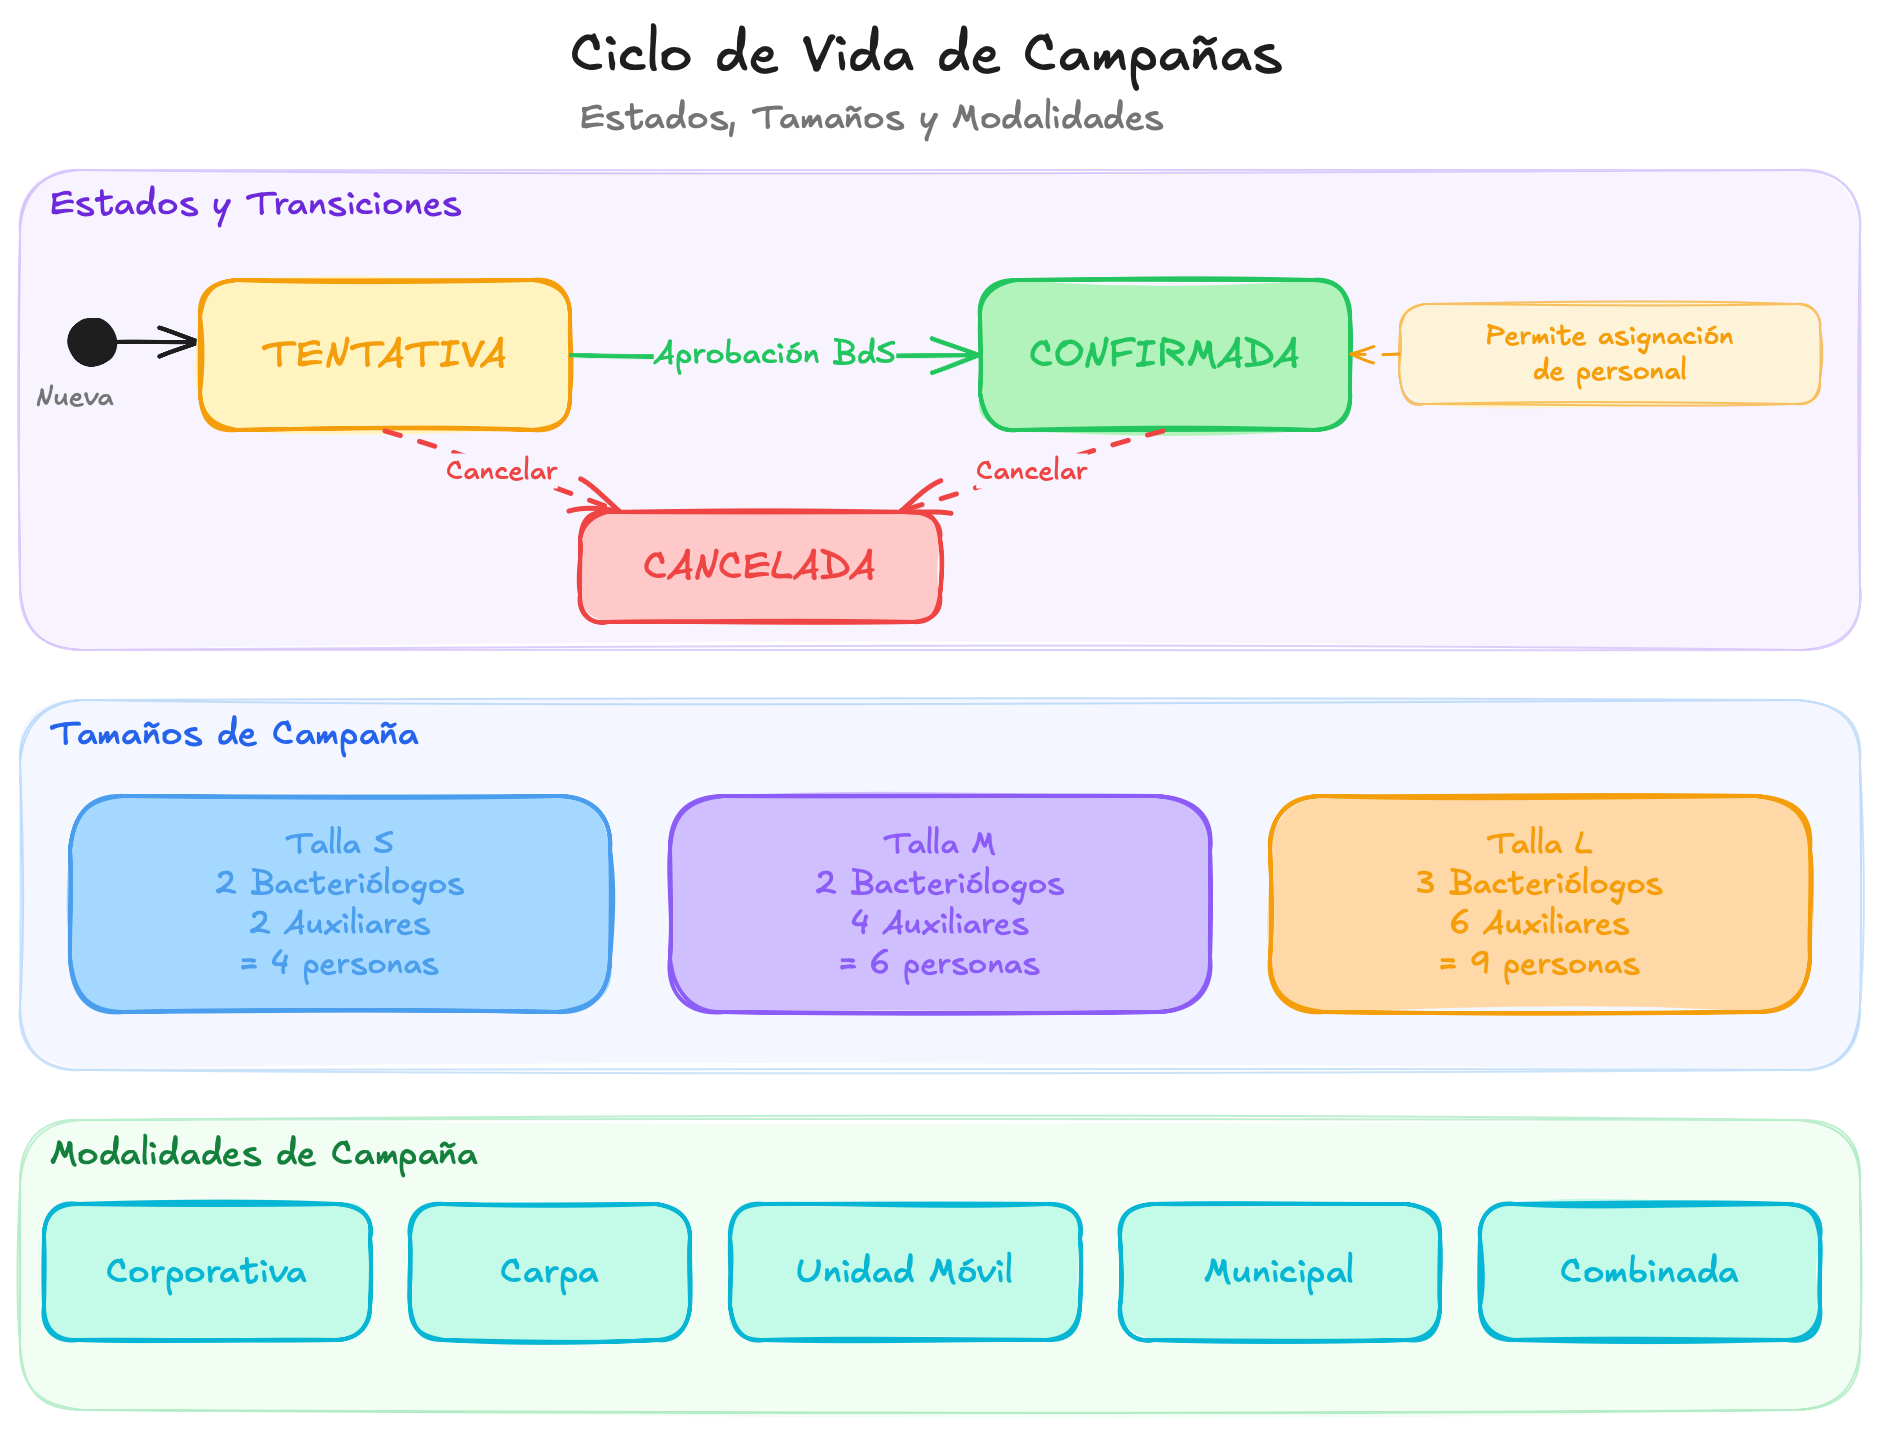
\includegraphics[width=0.92\textwidth]{Untitled-2026-02-11-1419.png}
\caption{Ciclo de vida de campañas: estados, transiciones, tamaños y modalidades}
\label{fig:ciclo-vida-campanas}
\end{figure}

\subsection{Coordinador de Campaña}

El coordinador de campaña \textbf{no es un cargo fijo}. Es una \textbf{responsabilidad que se asigna por cada campaña}:

\begin{itemize}[leftmargin=2em]
    \item Al programar una campaña, Banco de Sangre \textbf{designa a una persona del equipo asignado como coordinador} de esa campaña.
    \item El coordinador registra la \textbf{l\'{i}nea de tiempo completa} de la campaña y observaciones de campo (solo para esa campaña).
    \item Un empleado puede ser coordinador de una campaña y personal operativo en otra.
    \item El coordinador var\'{i}a de campaña en campaña; no es siempre la misma persona.
\end{itemize}

\subsubsection{L\'{i}nea de Tiempo de Campaña (Trazabilidad de Horas)}

El coordinador registra \textbf{todos los momentos} de la l\'{i}nea de tiempo para tener trazabilidad completa:

\begin{enumerate}[leftmargin=2em]
    \item \textbf{Hora de salida de sede:} El equipo parte de la sede principal.
    \item \textbf{Hora de llegada al punto:} Llegada al lugar de la campaña.
    \item \textbf{Hora de inicio de campaña:} Inicio de la atenci\'{o}n a donantes.
    \item \textbf{Hora de salida a almuerzo:} Inicio del receso.
    \item \textbf{Hora de regreso de almuerzo:} Fin del receso.
    \item \textbf{Hora de finalizaci\'{o}n de campaña:} Fin de la atenci\'{o}n a donantes.
    \item \textbf{Hora de recogida:} Recogida del equipo y material.
    \item \textbf{Hora de llegada a sede:} Regreso del equipo a sede.
    \item \textbf{Hora de salida de sede (fin):} El personal termina su jornada y sale de sede.
\end{enumerate}

\newpage
% ══════════════════════════════════════════════════════════════
\section{Perfiles de Personal}
% ══════════════════════════════════════════════════════════════

\subsection{Tipos de Perfil}

\begin{table}[h!]
\centering
\begin{tabularx}{\textwidth}{|l|l|X|}
\hline
\textbf{Perfil} & \textbf{Rol} & \textbf{Descripci\'{o}n} \\
\hline
Bacteri\'{o}logo & Operativo & Profesional responsable del proceso de extracci\'{o}n y manejo de hemocomponentes. Participa en campañas seg\'{u}n su \'{a}rea de entrenamiento. \\
\hline
M\'{e}dico & Operativo & Profesional m\'{e}dico que atiende a donantes. Se asigna seg\'{u}n necesidad espec\'{i}fica de cada campaña. \\
\hline
T\'{e}cnico Operativo & Operativo & Auxiliar de enfermer\'{i}a.\\
\hline
T\'{e}cnico Administrativo & Adm./Operativo & Personal administrativo que comenzar\'{a} a realizar turnos rotativos (completo, noche, posturno). \\
\hline
\end{tabularx}
\caption{Perfiles de personal del Banco de Sangre}
\end{table}

\subsection{\'{A}reas de Trabajo}

No todo el personal puede participar en todas las campañas. La habilitaci\'{o}n depende de su experiencia:

\begin{itemize}[leftmargin=2em]
    \item El sistema tiene un \textbf{cat\'{a}logo de \'{a}reas de trabajo} disponibles.
    \item Los administradores asignan a cada empleado las \'{a}reas en las que puede trabajar.
    \item Al asignar personal a una campaña, el sistema \textbf{solo muestra personal habilitado} para el \'{a}rea requerida.
    \item La habilitaci\'{o}n es editable en cualquier momento (se pueden agregar o quitar \'{a}reas).
\end{itemize}

% ══════════════════════════════════════════════════════════════
\section{Programaci\'{o}n: Sede y Campañas}
% ══════════════════════════════════════════════════════════════

El sistema gestiona \textbf{dos flujos de programaci\'{o}n} sobre el mismo pool de personal.

\subsection{Turnos en Sede Principal}

\begin{itemize}[leftmargin=2em]
    \item Programar turnos semanales de cada empleado en sede (horario de entrada y salida).
    \item Tipos de turno: completo (diurno), noche y posturno.
    \item Cuando un empleado es asignado a una campaña, sus horas en sede se ajustan autom\'{a}ticamente para ese d\'{i}a.
    \item Vista de ocupaci\'{o}n en sede: qui\'{e}n est\'{a} en sede, qui\'{e}n en campaña, qui\'{e}n libre.
\end{itemize}

\subsection{Campañas Extramurales}

El personal se asigna a campañas fuera de sede seg\'{u}n su perfil, \'{a}rea de entrenamiento y disponibilidad.

\subsection{C\'{o}mputo Integrado de Horas}

Las horas de \textbf{sede} y de \textbf{campaña} se suman para calcular el total semanal de cada empleado:

\begin{itemize}[leftmargin=2em]
    \item \textbf{Horas semanales} = horas en sede + horas en campaña.
    \item Si el total supera las \textbf{44 horas} contratadas, el excedente son \textbf{horas extras}.
    \item Si el total es menor a 44 horas, el empleado \textbf{le debe horas} a la organizaci\'{o}n (se compensan en la semana siguiente).
    \item Las horas pendientes se \textbf{compensan en la semana siguiente} (saldo positivo o negativo).
\end{itemize}

\begin{figure}[H]
\centering
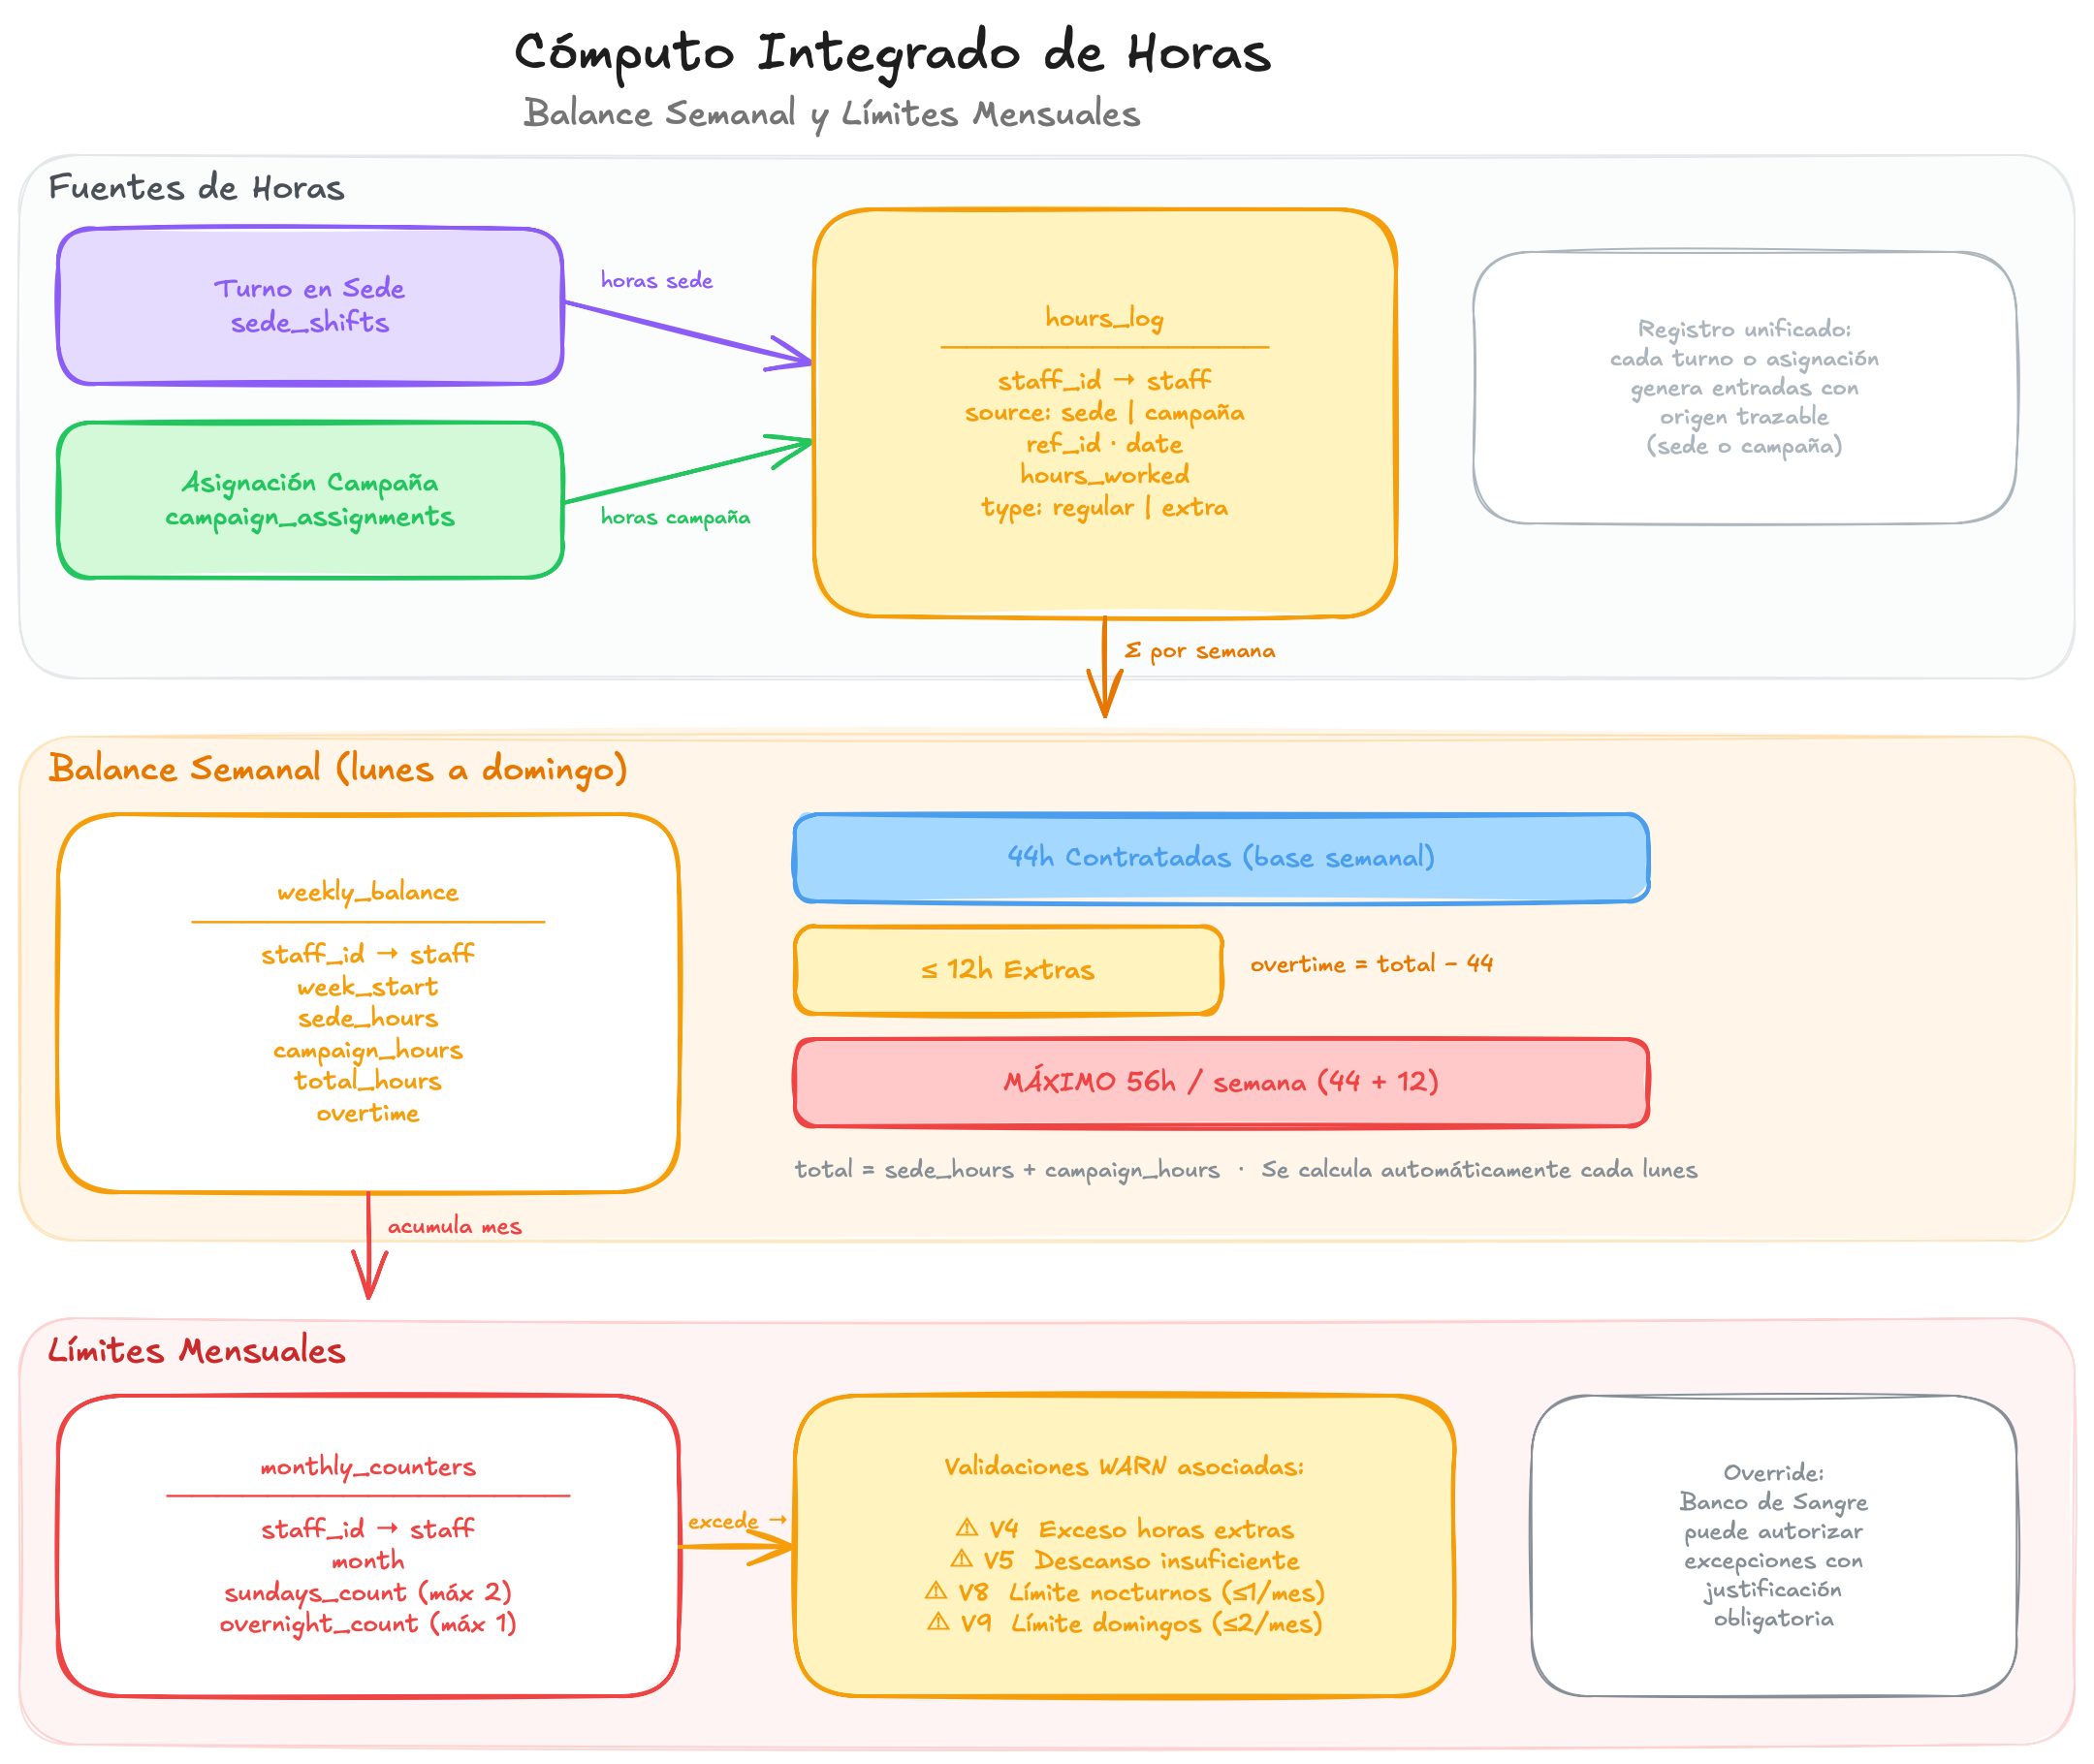
\includegraphics[width=\textwidth]{Untitled-2026-02-11-1419-8.png}
\caption{C\'{o}mputo integrado de horas: balance semanal (44h + 12h extras) y l\'{i}mites mensuales}
\label{fig:computo-horas}
\end{figure}


% ══════════════════════════════════════════════════════════════
\section{Reglas de Negocio}
% ══════════════════════════════════════════════════════════════

Todas las reglas son \textbf{configurables} desde el sistema (se pueden ajustar ante cambios normativos sin intervenci\'{o}n t\'{e}cnica).

\subsection{L\'{i}mites Semanales}

\begin{table}[h!]
\centering
\begin{tabularx}{\textwidth}{|l|X|c|}
\hline
\textbf{Regla} & \textbf{Descripci\'{o}n} & \textbf{Valor actual} \\
\hline
Jornada semanal & Horas ordinarias semanales por contrato & 44 horas \\
\hline
M\'{a}x. horas extras/semana & L\'{i}mite de horas extra por empleado por semana & 12 horas \\
\hline
M\'{a}x. horas por turno & Duraci\'{o}n m\'{a}xima de un turno continuo & 12 horas \\
\hline
Descanso entre turnos & Horas de descanso obligatorio entre jornadas & 8 horas \\
\hline
\end{tabularx}
\caption{L\'{i}mites semanales configurables}
\end{table}

\subsection{L\'{i}mites Mensuales}

\begin{table}[h!]
\centering
\begin{tabularx}{\textwidth}{|l|X|c|}
\hline
\textbf{Regla} & \textbf{Descripci\'{o}n} & \textbf{Valor actual} \\
\hline
M\'{a}x. domingos por mes & Domingos trabajados por empleado al mes & 2 \\
\hline
M\'{a}x. pernoctas por mes & Pernoctas por empleado al mes & 1 \\
\hline
\end{tabularx}
\caption{L\'{i}mites mensuales configurables}
\end{table}

\textbf{Restricciones de domingos:}
\begin{itemize}[leftmargin=2em]
    \item \textbf{Para Comercial:} Solo pueden programar campañas \textbf{m\'{a}ximo dos domingos al mes} en total.
    \item \textbf{Para el personal:} El sistema genera una \textbf{alerta} cuando un empleado haya trabajado dos domingos en el mes, impidiendo asignarlo a un tercer domingo.
\end{itemize}

\subsection{Restricciones de Municipios y Pernoctas}

Cuando el personal se desplaza a \textbf{municipios diferentes} a la sede principal:

\begin{itemize}[leftmargin=2em]
    \item \textbf{D\'{i}a anterior a campaña municipal:} No se le deben programar campañas el d\'{i}a anterior. Si tiene jornada regular, debe terminar \textbf{m\'{a}ximo a las 5:00 PM}.
    \item \textbf{D\'{i}a anterior a pernocta:} Misma restricci\'{o}n: no campañas el d\'{i}a previo; jornada regular m\'{a}ximo hasta las 5:00 PM.
    \item El sistema valida estas restricciones \textbf{autom\'{a}ticamente} al asignar personal.
\end{itemize}

\subsection{Validaciones al Asignar Personal}

Cuando se intenta asignar una persona a una campaña, el sistema realiza \textbf{9 validaciones autom\'{a}ticas}. Tres de ellas \textbf{impiden} la asignaci\'{o}n (bloqueos duros) y seis generan \textbf{advertencias} que requieren criterio humano:

\begin{table}[h!]
\centering
\small
\begin{tabularx}{\textwidth}{|c|l|c|X|}
\hline
\textbf{\#} & \textbf{Situaci\'{o}n} & \textbf{Acci\'{o}n} & \textbf{Descripci\'{o}n} \\
\hline
\rowcolor{rojoclaro}
1 & Superposici\'{o}n horaria & \textbf{IMPIDE} & Ya asignado a otra actividad en el mismo horario \\
\hline
\rowcolor{rojoclaro}
2 & Turno excesivo & \textbf{IMPIDE} & El turno superar\'{i}a 12 horas continuas \\
\hline
\rowcolor{rojoclaro}
3 & \'{A}rea no habilitada & \textbf{IMPIDE} & No est\'{a} capacitado para el \'{a}rea de la campaña \\
\hline
\rowcolor{amarilloclaro}
4 & Exceso horas extras & ADVIERTE & Excedr\'{i}a las 12 horas extras semanales \\
\hline
\rowcolor{amarilloclaro}
5 & No disponible & ADVIERTE & Marcado como no disponible \\
\hline
\rowcolor{amarilloclaro}
6 & Descanso insuficiente & ADVIERTE & Menos de 8 horas entre turnos \\
\hline
\rowcolor{amarilloclaro}
7 & L\'{i}mite domingos & ADVIERTE & Ya trabaj\'{o} 2 domingos este mes \\
\hline
\rowcolor{amarilloclaro}
8 & L\'{i}mite pernoctas & ADVIERTE & Ya tuvo 1 pernocta este mes \\
\hline
\rowcolor{amarilloclaro}
9 & Restricci\'{o}n municipio & ADVIERTE & Tiene actividad el d\'{i}a anterior que termina despu\'{e}s de 5pm \\
\hline
\end{tabularx}
\caption{Las 9 validaciones al asignar personal (\colorbox{rojoclaro}{rojo} = bloqueo, \colorbox{amarilloclaro}{amarillo} = advertencia)}
\end{table}

\begin{figure}[H]
\centering
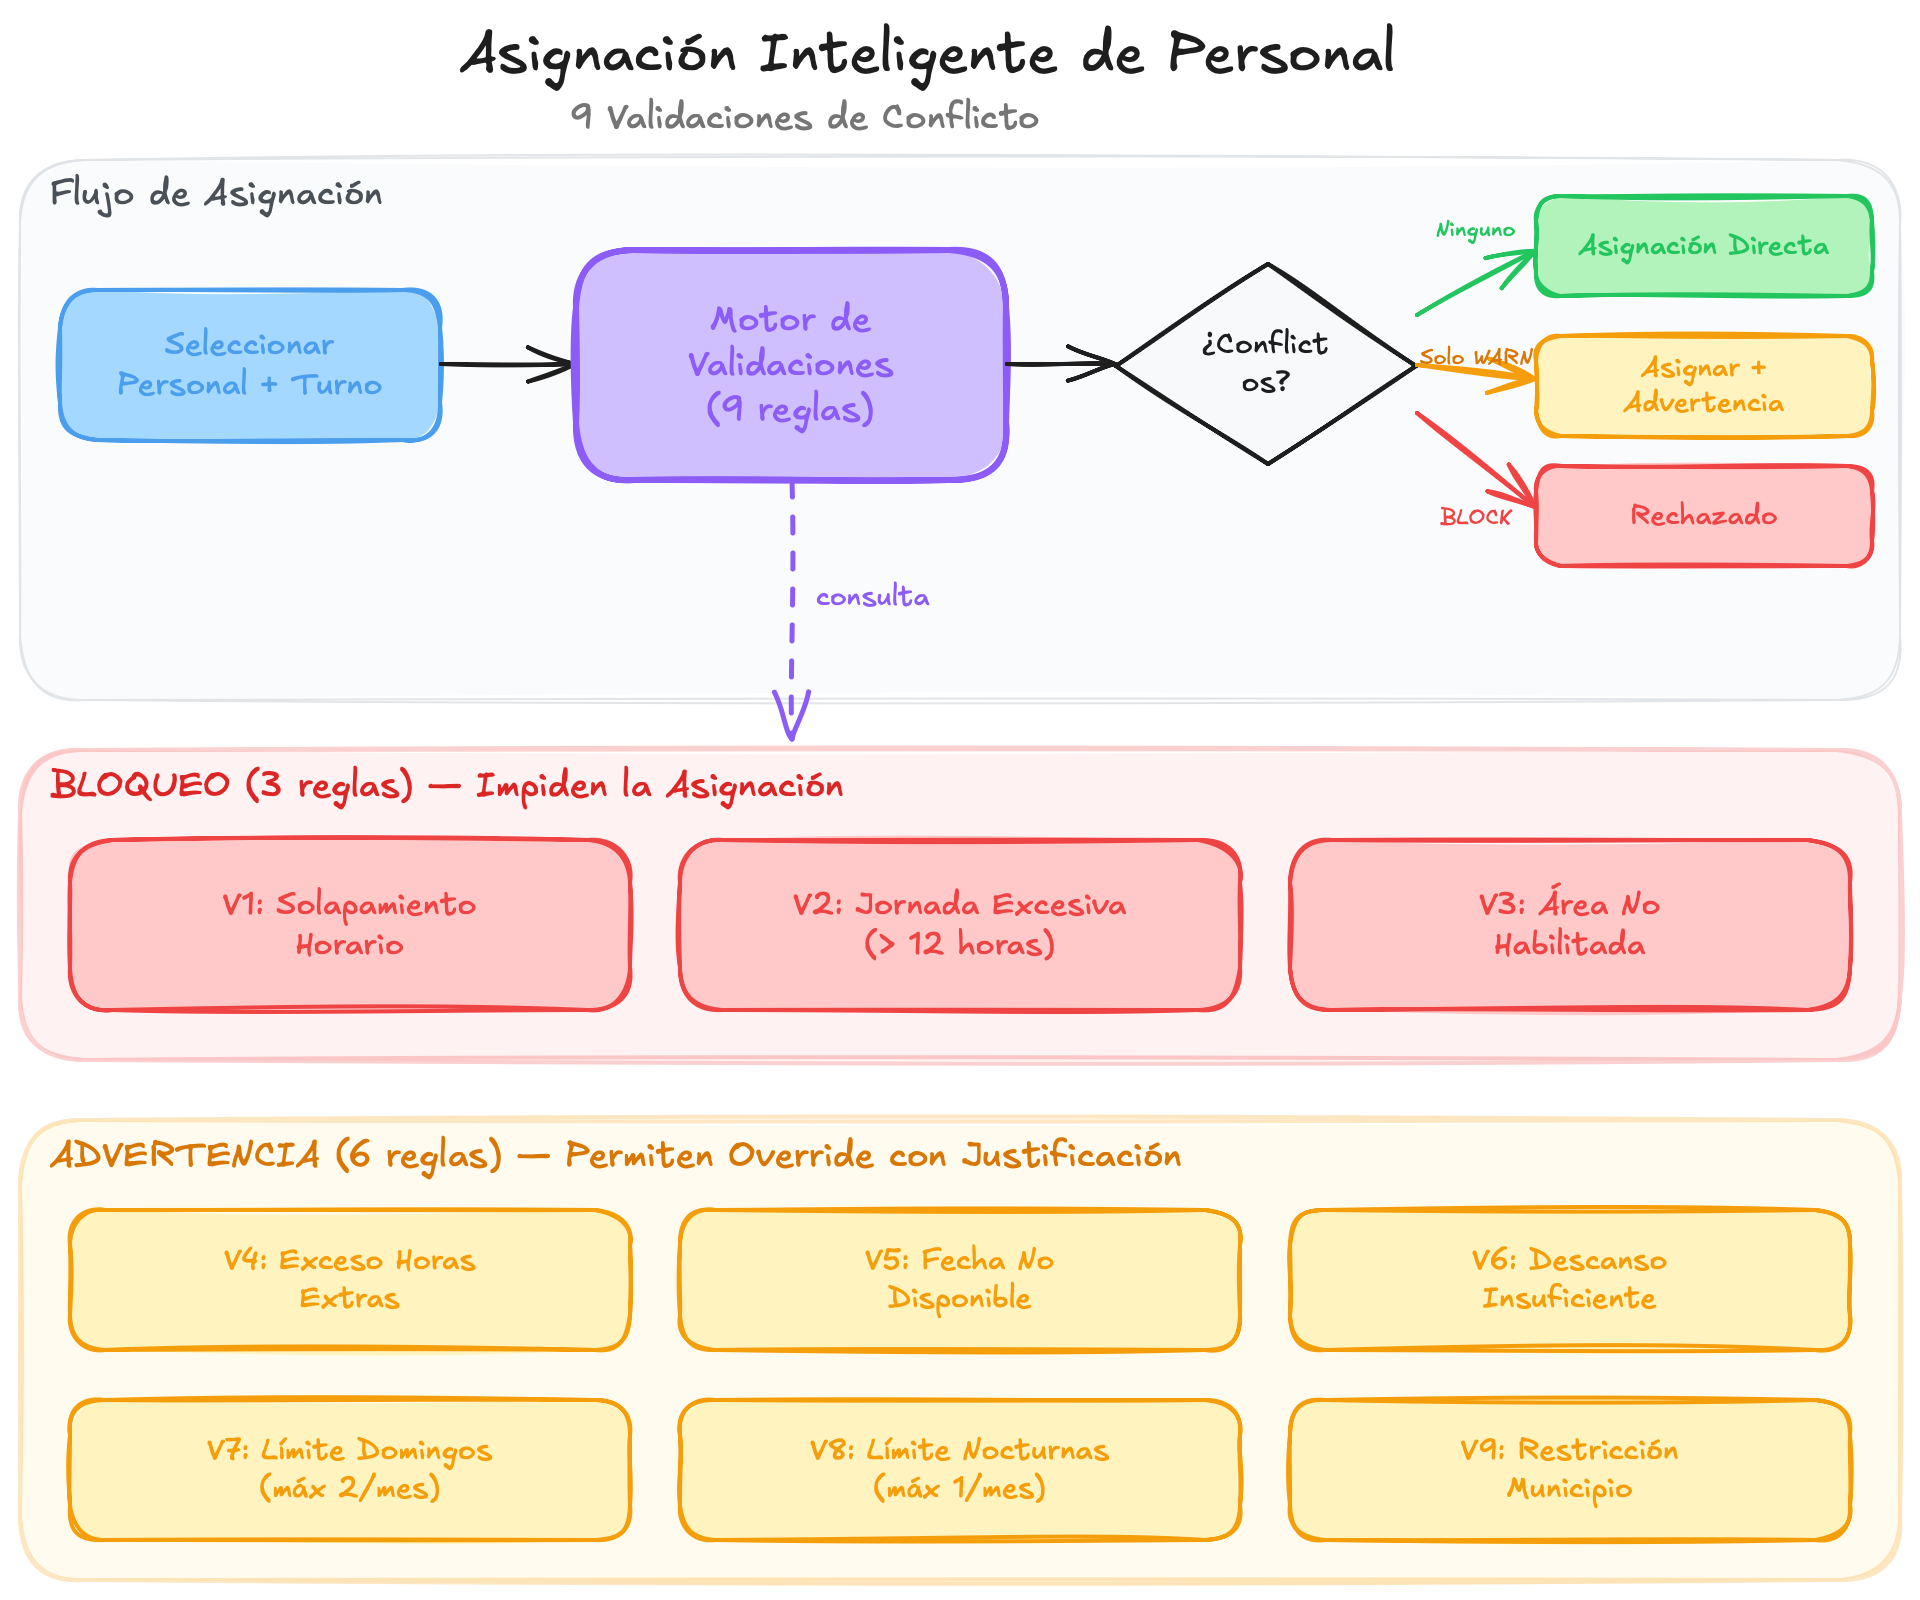
\includegraphics[width=0.85\textwidth]{Untitled-2026-02-11-1419-3.png}
\caption{Flujo de asignaci\'{o}n inteligente: motor de 9 validaciones}
\label{fig:asignacion-inteligente}
\end{figure}

\subsection{Balance Semanal de Horas}

El sistema lleva un \textbf{registro semanal por persona} que indica:

\begin{table}[h!]
\centering
\begin{tabularx}{\textwidth}{|l|X|}
\hline
\textbf{Estado} & \textbf{Significado} \\
\hline
\rowcolor{verdeclaro}
\textbf{Cumpli\'{o}} & Trabaj\'{o} exactamente 44 horas. \\
\hline
\textbf{Horas extras} & Trabaj\'{o} m\'{a}s de 44 horas. El excedente se registra como extras. \\
\hline
\textbf{Debe horas} & Trabaj\'{o} menos de 44 horas. El empleado debe compensar esas horas a la organizaci\'{o}n en la semana siguiente. \\
\hline
\end{tabularx}
\caption{Estados del balance semanal}
\end{table}

Las horas pendientes se \textbf{arrastran a la semana siguiente} como saldo positivo o negativo.

\textbf{Ejemplo:}

\small
\begin{tabular}{|l|l|c|c|c|c|c|}
\hline
\textbf{Empleado} & \textbf{Perfil} & \textbf{Sede} & \textbf{Campaña} & \textbf{Total} & \textbf{Extras} & \textbf{Balance} \\
\hline
J. P\'{e}rez & Bact. & 36h & 8h & 44h & 0h & Cumpli\'{o} \\
\hline
M. L\'{o}pez & T\'{e}c.Op. & 44h & 14h & 58h & \textcolor{red}{14h} & +14h extras \\
\hline
A. G\'{o}mez & T\'{e}c.Adm. & 38h & 0h & 38h & 0h & Debe 6h \\
\hline
R. D\'{i}az & Bact. & 24h & 16h & 40h & 0h & Debe 4h \\
\hline
\end{tabular}
\normalsize


% ══════════════════════════════════════════════════════════════
\section{Integraciones Externas}
% ══════════════════════════════════════════════════════════════

\subsection{Flujo CRM $\rightarrow$ Excel $\rightarrow$ Plataforma}

El equipo comercial \textbf{busca activamente} campañas (es un proceso de venta). El flujo semanal es:

\begin{enumerate}[leftmargin=2em]
    \item \textbf{Comercial} gestiona y concreta campañas con empresas/organizaciones.
    \item Registra la campaña en el \textbf{CRM}.
    \item Exporta la informaci\'{o}n a un \textbf{archivo Excel}.
    \item Sube el Excel \textbf{semanalmente} a la plataforma. Las campañas se crean en estado \textbf{tentativa}.
    \item \textbf{Comercial} revisa y \textbf{confirma} las campañas en la plataforma (estado pasa a \textbf{confirmada}).
    \item Banco de Sangre \textbf{asigna el personal} a las campañas confirmadas, seg\'{u}n las reglas del sistema.
    \item Comercial puede \textbf{consultar en la plataforma} los datos de personal asignado.
\end{enumerate}

\begin{figure}[H]
\centering
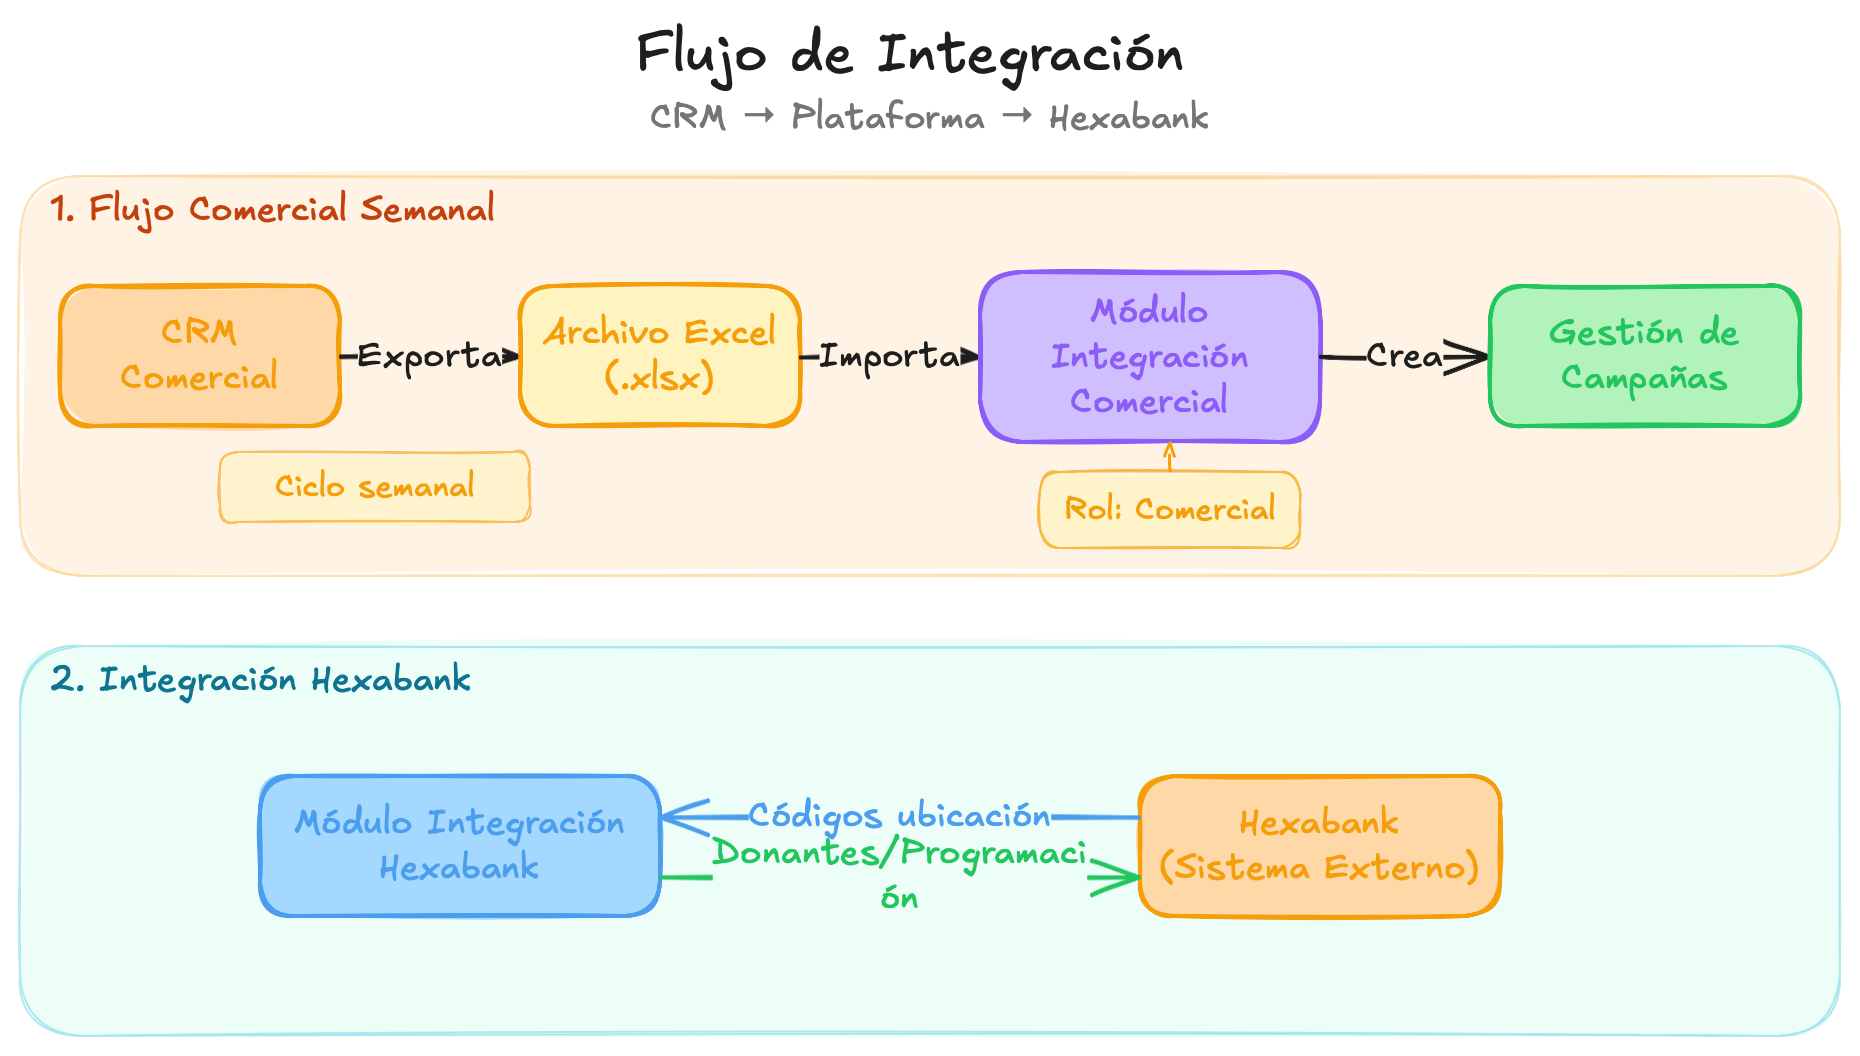
\includegraphics[width=0.88\textwidth]{Untitled-2026-02-11-1419-4.png}
\caption{Flujo de integraci\'{o}n: CRM $\rightarrow$ Excel $\rightarrow$ Plataforma $\rightarrow$ Hexabank}
\label{fig:flujo-integracion}
\end{figure}

\subsection{Datos del Excel de Importaci\'{o}n (desde CRM)}

\begin{table}[h!]
\centering
\begin{tabularx}{\textwidth}{|l|X|}
\hline
\textbf{Campo} & \textbf{Descripci\'{o}n} \\
\hline
C\'{o}digo & Identificador \'{u}nico de la campaña (del CRM) \\
\hline
Nombre de la empresa & Empresa u organizaci\'{o}n donde se realizar\'{a} la campaña \\
\hline
Municipio & Municipio donde se realizar\'{a} \\
\hline
Mix (tamaño) & S, M o L \\
\hline
Fecha & Fecha programada \\
\hline
Modalidad & Corporativa, carpa, unidad m\'{o}vil, municipal, combinada \\
\hline
Observaciones & Campo libre para notas \\
\hline
\end{tabularx}
\caption{Campos del archivo Excel de importaci\'{o}n}
\end{table}

\subsection{Datos que Consulta Comercial en la Plataforma}

Una vez que Banco de Sangre asigna el personal a la campaña (registrada por Comercial), Comercial puede ver:

\begin{itemize}[leftmargin=2em]
    \item C\'{o}digo y nombre de la empresa.
    \item Municipio, fecha y modalidad.
    \item \textbf{Personal asignado:} nombre completo, n\'{u}mero de c\'{e}dula y cargo.
    \item Estado de la campaña (tentativa, confirmada, cancelada).
\end{itemize}

\subsection{Integraci\'{o}n con Hexabank}

Hexabank es el sistema de gesti\'{o}n del Banco de Sangre. Se requieren dos datos:

\begin{itemize}[leftmargin=2em]
    \item \textbf{C\'{o}digo de lugar:} Cada punto de recolecci\'{o}n tiene un c\'{o}digo en Hexabank. La plataforma permite relacionar cada campaña con su c\'{o}digo.
    \item \textbf{Datos de donantes:} Horas y fechas de donaci\'{o}n para an\'{a}lisis y seguimiento.
\end{itemize}

En la primera fase, esta integraci\'{o}n ser\'{a} \textbf{manual} (campo de texto para el c\'{o}digo). En fases posteriores se puede automatizar.

\subsection{Migraci\'{o}n de Directorio de Contactos}

Comercial requiere migrar su \textbf{base de datos de directorio} (contactos de empresas, organizaciones, responsables) a la plataforma.

% ══════════════════════════════════════════════════════════════
\section{Roles y Permisos}
% ══════════════════════════════════════════════════════════════

El sistema define \textbf{cuatro roles} con permisos diferenciados:

\begin{figure}[H]
\centering
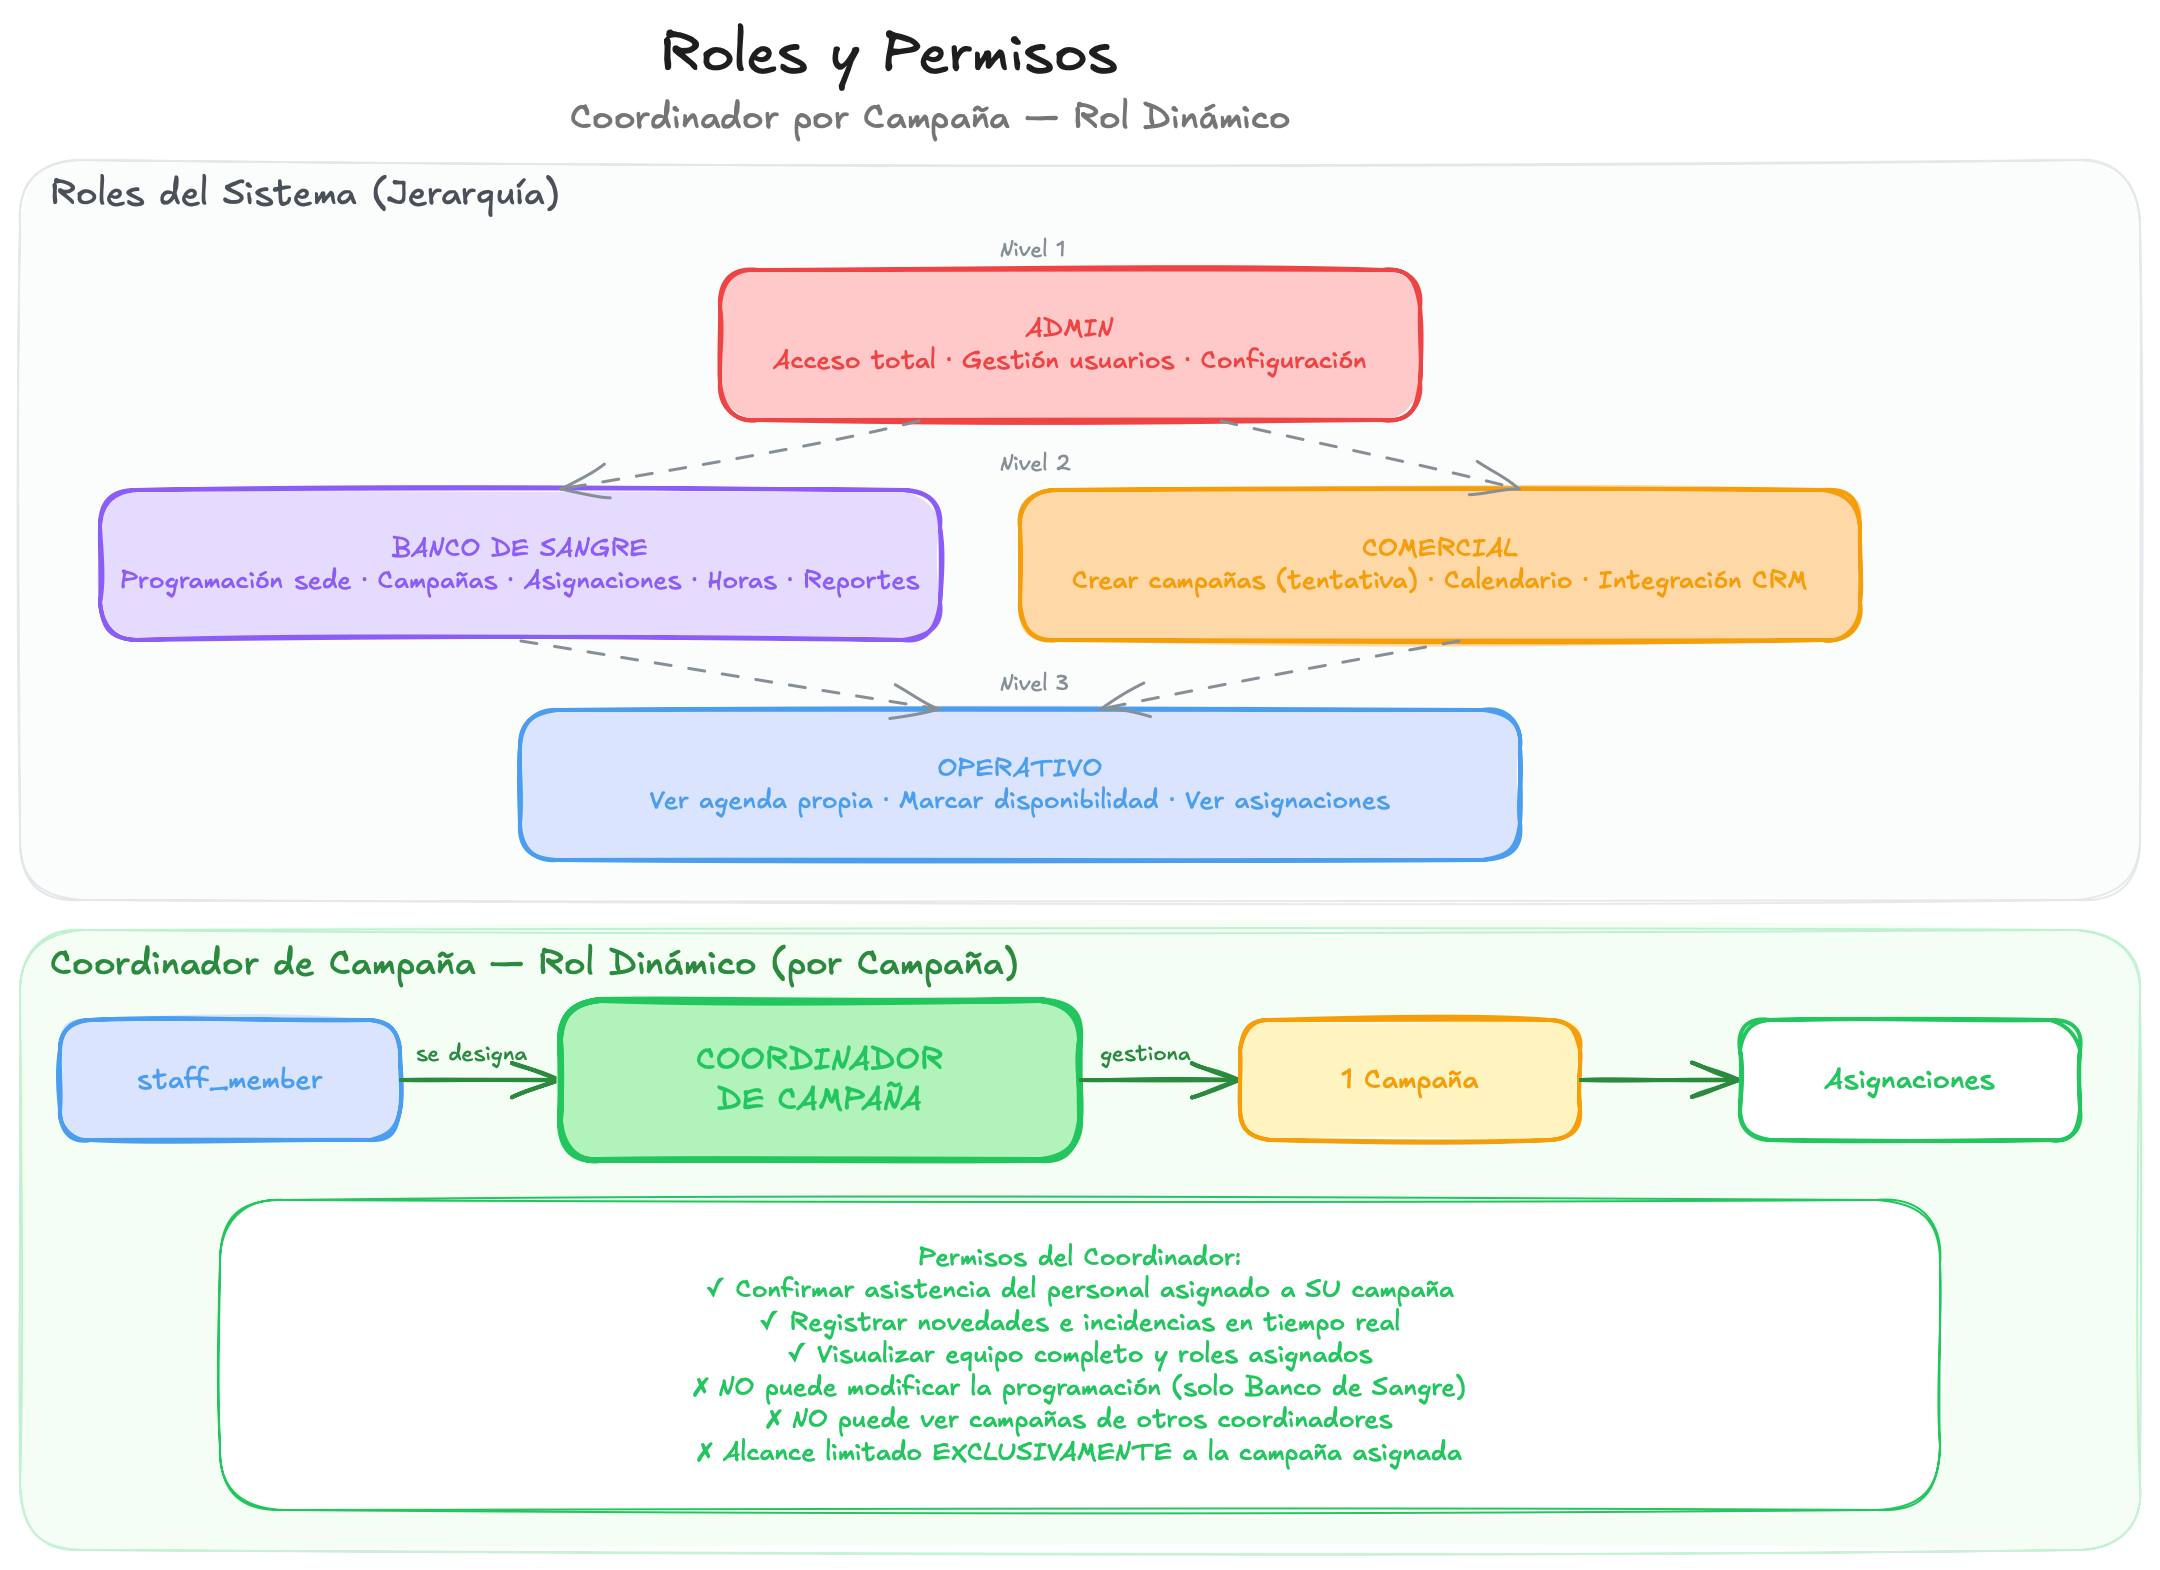
\includegraphics[width=0.92\textwidth]{Untitled-2026-02-11-1419-7.png}
\caption{Jerarqu\'{i}a de roles del sistema + coordinador de campaña (designaci\'{o}n din\'{a}mica)}
\label{fig:roles-permisos}
\end{figure}

\begin{table}[h!]
\centering
\small
\begin{tabularx}{\textwidth}{|X|c|c|c|c|}
\hline
\textbf{?`Qu\'{e} puede hacer?} & \textbf{Admin} & \textbf{B. Sangre} & \textbf{Comercial} & \textbf{Operativo} \\
\hline
Ver dashboard general & S\'{i} & S\'{i} & S\'{i} & Solo personal \\
\hline
Crear y editar personal & S\'{i} & S\'{i} & --- & --- \\
\hline
Programar turnos en sede & S\'{i} & S\'{i} & --- & --- \\
\hline
Crear y editar campañas & S\'{i} & --- & S\'{i} & --- \\
\hline
Confirmar/cancelar campañas & S\'{i} & --- & S\'{i} & --- \\
\hline
Ver campañas & S\'{i} & S\'{i} & S\'{i} & Solo asignadas \\
\hline
Asignar personal a campañas & S\'{i} & S\'{i} & --- & --- \\
\hline
Cargar Excel desde CRM & S\'{i} & S\'{i} & S\'{i} & --- \\
\hline
Ver personal asignado & S\'{i} & S\'{i} & Nombre, CC, cargo & --- \\
\hline
Registrar hora real de campaña & S\'{i} & S\'{i} & --- & Solo como coordinador \\
\hline
Ver disponibilidad de personal & S\'{i} & S\'{i} & Resumen & Solo propia \\
\hline
Ver reportes de horas & S\'{i} & S\'{i} & --- & Solo propias \\
\hline
Ver reportes de campañas & S\'{i} & S\'{i} & S\'{i} & --- \\
\hline
Configurar el sistema & S\'{i} & --- & --- & --- \\
\hline
\end{tabularx}
\caption{?`Qu\'{e} puede hacer cada rol en el sistema?}
\end{table}

\newpage

% ══════════════════════════════════════════════════════════════
\section{Flujos de Trabajo Paso a Paso}
% ══════════════════════════════════════════════════════════════

\subsection{Flujo 1: Carga y Confirmaci\'{o}n de Campañas}

\textbf{Responsable: Comercial $\rightarrow$ Banco de Sangre}

\begin{enumerate}[leftmargin=2em]
    \item \textbf{Comercial} concreta campañas con empresas y las registra en el CRM.
    \item Semanalmente, exporta los datos a un archivo Excel.
    \item Sube el Excel a la plataforma.
    \item El sistema valida los datos y crea las campañas como \textbf{tentativas}.
    \item \textbf{Comercial} revisa las campañas importadas, ajusta si es necesario y las \textbf{confirma} (estado pasa a \textbf{confirmada}).
    \item \textbf{Banco de Sangre} recibe las campañas confirmadas y procede con la \textbf{asignaci\'{o}n de personal}.
\end{enumerate}

\subsection{Flujo 2: Asignaci\'{o}n de Personal a Campaña}

\textbf{Responsable: Banco de Sangre}

\begin{enumerate}[leftmargin=2em]
    \item Abre una campaña confirmada.
    \item El sistema muestra los requerimientos seg\'{u}n el tamaño (ej: M = 2 bacteri\'{o}logos + 4 t\'{e}cnicos).
    \item Selecciona ``Asignar Personal''. El sistema muestra un panel con:
    \begin{itemize}
        \item Personal filtrado por perfil requerido \textbf{y} \'{a}rea habilitada.
        \item Personal con conflictos excluido autom\'{a}ticamente.
        \item Indicadores de horas extras, domingos y pernoctas de cada candidato.
        \item Sem\'{a}foro de colores: \textcolor{green!70!black}{verde} (disponible), \textcolor{yellow!80!black}{amarillo} (cerca del l\'{i}mite), \textcolor{red}{rojo} (al l\'{i}mite).
    \end{itemize}
    \item Selecciona personal. El sistema \textbf{bloquea o advierte} seg\'{u}n las 9 validaciones.
    \item Confirma asignaciones.
    \item \textbf{Designa coordinador} de entre el personal asignado.
    \item Comercial puede ver el personal asignado (nombre, c\'{e}dula, cargo).
\end{enumerate}

\subsection{Flujo 3: Programaci\'{o}n de Turnos en Sede}

\textbf{Responsable: Banco de Sangre}

\begin{enumerate}[leftmargin=2em]
    \item Navega al m\'{o}dulo de ``Programaci\'{o}n en Sede''.
    \item Selecciona la semana a programar.
    \item Asigna turnos a cada empleado: d\'{i}a, tipo de turno, hora de inicio y fin.
    \item El sistema valida que no haya conflictos con campañas asignadas ese d\'{i}a.
    \item Las horas de sede se suman al balance semanal de cada empleado.
    \item Si un empleado es asignado a campaña, su turno de sede se ajusta autom\'{a}ticamente.
\end{enumerate}

\subsection{Flujo 4: Registro de Horas Reales en Campaña}

\textbf{Responsable: Coordinador de campaña (designado)}

\begin{enumerate}[leftmargin=2em]
    \item La campaña tiene hora de inicio programada y hora estimada de fin.
    \item El coordinador asiste a la jornada.
    \item Durante y al finalizar la campaña, registra la \textbf{l\'{i}nea de tiempo completa}: hora de salida de sede, llegada al punto, inicio de campaña, almuerzo, finalizaci\'{o}n, recogida, llegada a sede y salida de sede, junto con observaciones.
    \item Solo puede registrar datos de \textbf{su campaña asignada} (no de otras).
    \item El sistema calcula las horas reales a partir de la l\'{i}nea de tiempo y actualiza el balance de todo el equipo.
\end{enumerate}

\subsection{Flujo 5: Monitoreo Semanal de Horas}

\textbf{Responsable: Admin / Banco de Sangre}

\begin{enumerate}[leftmargin=2em]
    \item Navega a ``Reporte de Horas'' y selecciona la semana.
    \item Ve una tabla con: horas en sede, horas en campaña, total, extras y balance de cada persona.
    \item Filas codificadas por color seg\'{u}n porcentaje del l\'{i}mite.
    \item Puede exportar el reporte a Excel.
\end{enumerate}

\subsection{Flujo 6: Lo que Ve el Personal Operativo}

\textbf{Responsable: Cada empleado}

\begin{enumerate}[leftmargin=2em]
    \item Inicia sesi\'{o}n y ve su dashboard personal.
    \item Ve su \textbf{calendario integrado}: turnos en sede + campañas asignadas.
    \item Ve resumen de horas de la semana y balance acumulado.
    \item Ve contadores del mes: domingos trabajados y pernoctas.
    \item Si fue designado coordinador, ve acceso directo para registrar horas reales.
    \item Puede marcar fechas como no disponible con motivo.
\end{enumerate}

\subsection{Flujo 7: Cancelaci\'{o}n de Campaña}

\textbf{Responsable: Comercial} (es quien establece el contacto directo con la empresa).

\begin{enumerate}[leftmargin=2em]
    \item \textbf{Comercial} abre el detalle de la campaña y selecciona ``Cancelar''.
    \item Ingresa motivo de cancelaci\'{o}n (obligatorio).
    \item El sistema muestra personal afectado y horas que se liberar\'{a}n.
    \item Al confirmar: asignaciones anuladas, estado cambia a \textit{cancelada}.
    \item Banco de Sangre es notificado de la cancelaci\'{o}n para ajustar la programaci\'{o}n del personal.
    \item Queda registrado en log de auditor\'{i}a.
\end{enumerate}

\newpage
% ══════════════════════════════════════════════════════════════
\section{Visi\'{o}n General de la Plataforma}
% ══════════════════════════════════════════════════════════════

\begin{figure}[H]
\centering
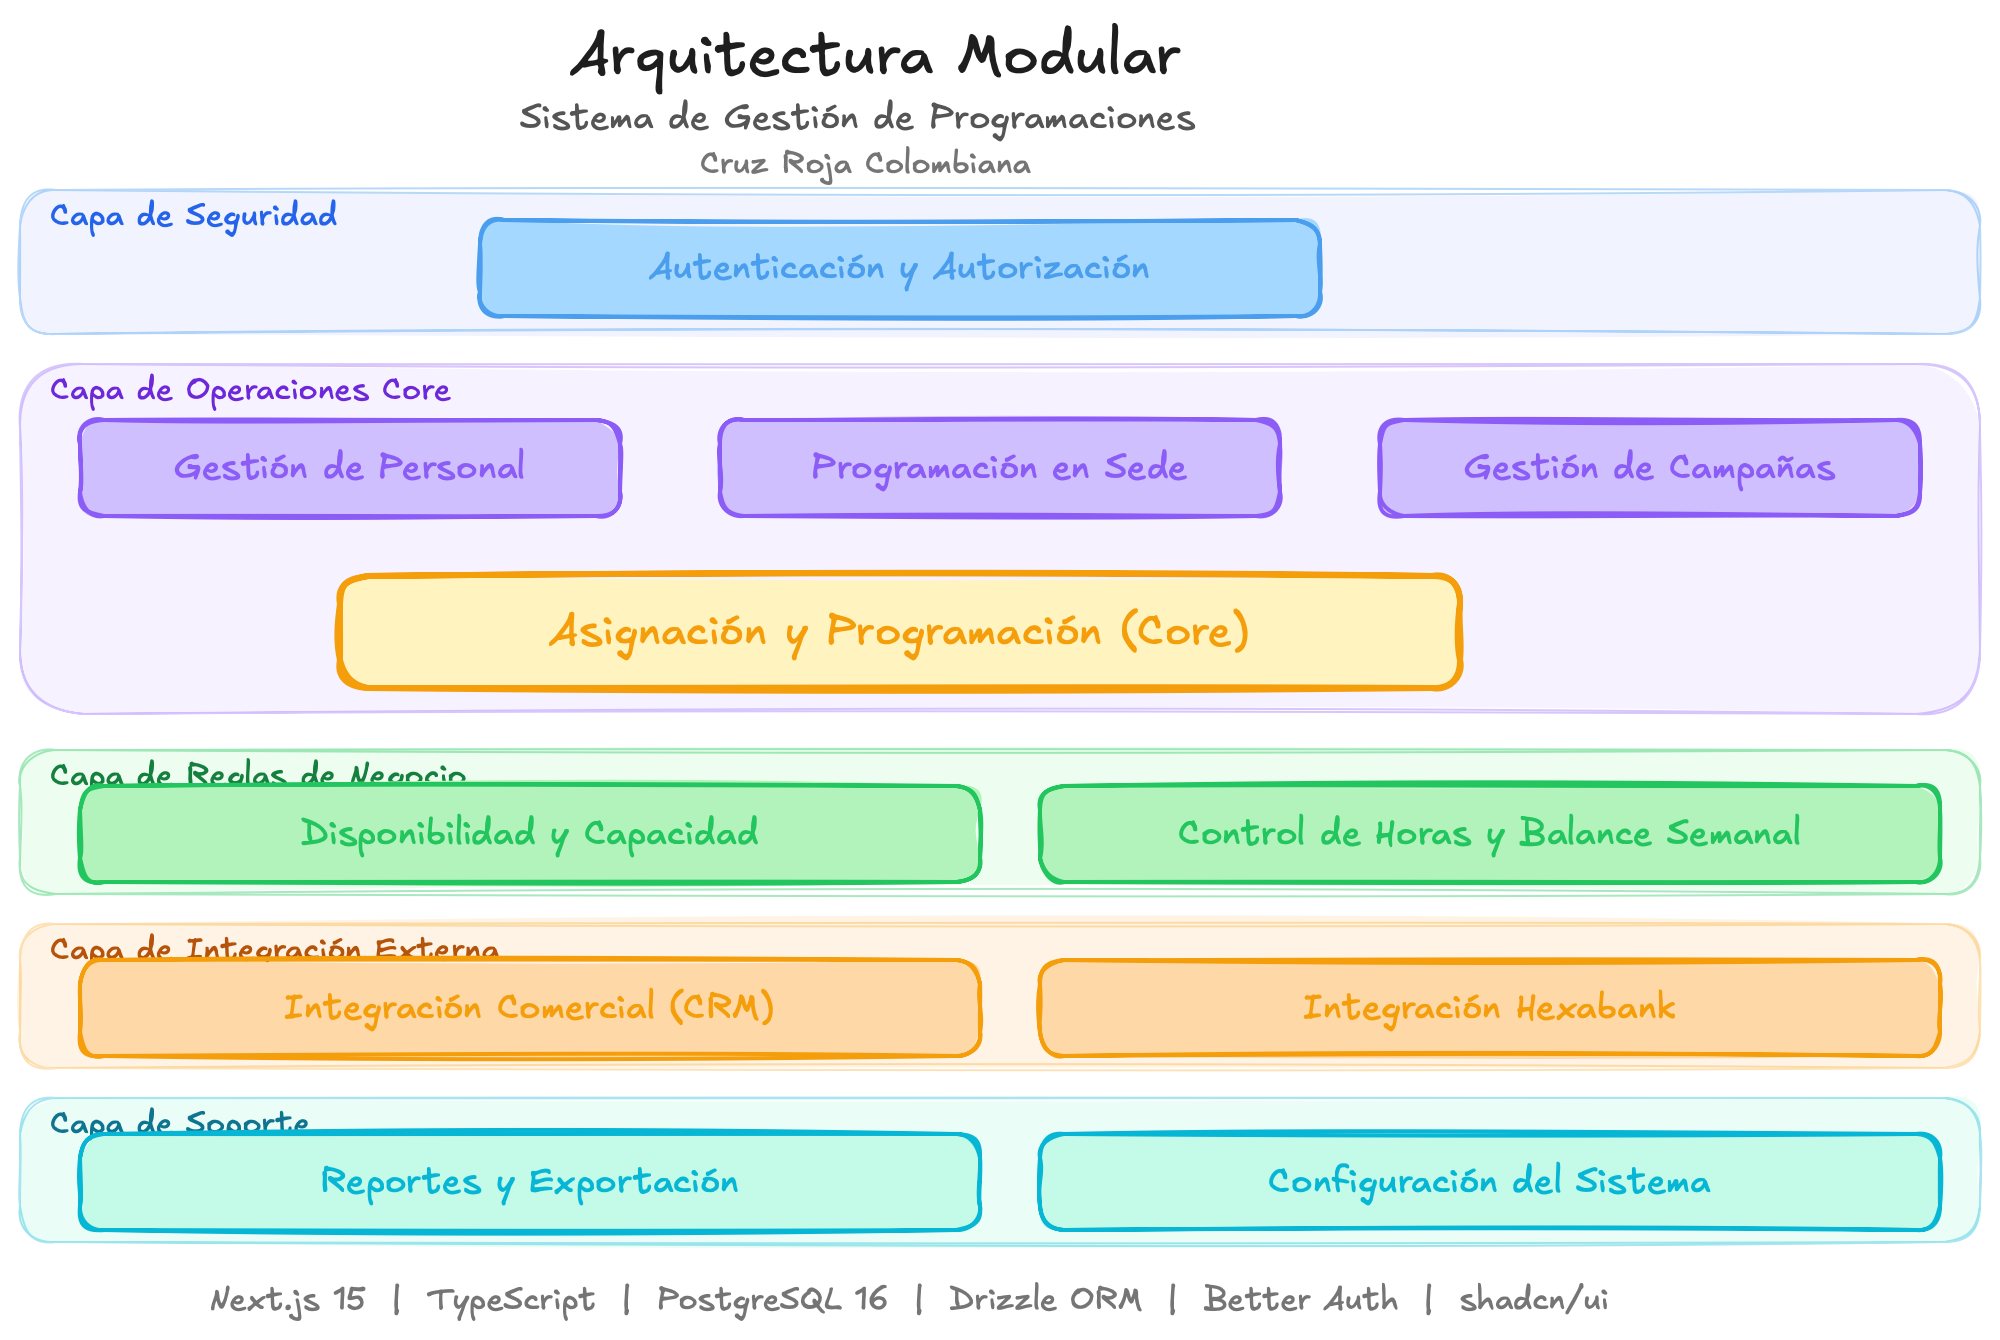
\includegraphics[width=0.92\textwidth]{Untitled-2026-02-11-1419-6.png}
\caption{Arquitectura del sistema: m\'{o}dulos principales organizados por funci\'{o}n}
\label{fig:arquitectura-modular}
\end{figure}

La plataforma se organiza en los siguientes m\'{o}dulos funcionales:

\begin{enumerate}[leftmargin=2em]
    \item \textbf{Acceso y seguridad:} Login, control de permisos por rol.
    \item \textbf{Gesti\'{o}n de personal:} Directorio de empleados, perfiles, \'{a}reas de trabajo habilitadas.
    \item \textbf{Programaci\'{o}n en sede:} Turnos semanales en sede principal.
    \item \textbf{Gesti\'{o}n de campañas:} Crear, editar, confirmar y cancelar campañas con sus datos completos.
    \item \textbf{Asignaci\'{o}n inteligente:} Asignar personal con validaciones autom\'{a}ticas y sem\'{a}foro de horas.
    \item \textbf{Disponibilidad y capacidad:} Ver qui\'{e}n est\'{a} disponible, calendario de capacidad para Comercial.
    \item \textbf{Control de horas:} Balance semanal, horas extras, contadores mensuales.
    \item \textbf{Integraci\'{o}n comercial:} Carga de Excel desde CRM, consulta de personal asignado.
    \item \textbf{Integraci\'{o}n Hexabank:} C\'{o}digos de lugar y datos de donantes.
    \item \textbf{Reportes:} Horas, campañas, extras, domingos, pernoctas. Exportables a Excel.
    \item \textbf{Configuraci\'{o}n:} Par\'{a}metros laborales, cat\'{a}logos, festivos, usuarios.
\end{enumerate}

\newpage

% ══════════════════════════════════════════════════════════════
\section{Plan de Implementaci\'{o}n}
% ══════════════════════════════════════════════════════════════

El desarrollo se organiza en \textbf{4 fases de 4 semanas} cada una:

\subsection{Fase 1 --- Sistema B\'{a}sico (Semanas 1--4)}

\begin{itemize}[leftmargin=2em]
    \item Login y control de acceso por roles.
    \item Directorio de personal con los 4 perfiles y \'{a}reas de trabajo.
    \item Programaci\'{o}n de turnos en sede.
    \item Gesti\'{o}n de campañas (3 estados, 3 tamaños, 5 modalidades).
    \item Asignaci\'{o}n b\'{a}sica de personal con designaci\'{o}n de coordinador.
    \item Importaci\'{o}n de campañas desde Excel (CRM).
    \item Dashboard general con navegaci\'{o}n por rol.
\end{itemize}

\subsection{Fase 2 --- Validaciones y Control (Semanas 5--8)}

\begin{itemize}[leftmargin=2em]
    \item Control de horas: registro de hora real por coordinador, balance semanal.
    \item Asignaci\'{o}n inteligente con las 9 validaciones autom\'{a}ticas.
    \item Contadores mensuales (domingos y pernoctas).
    \item Sem\'{a}foro de horas extras.
    \item Disponibilidad: matriz visual y calendario de capacidad.
    \item Flujo comercial completo: carga Excel + vista de personal asignado.
    \item Directorio de empresas y contactos.
\end{itemize}

\subsection{Fase 3 --- Reportes (Semanas 9--12)}

\begin{itemize}[leftmargin=2em]
    \item Reportes de horas con balance semanal, campañas, extras, domingos y pernoctas.
    \item Exportaci\'{o}n de todos los reportes a Excel.
    \item Importaci\'{o}n de datos desde Excel (personal, \'{a}reas, campañas).
    \item Log de auditor\'{i}a.
    \item Integraci\'{o}n de datos de Hexabank (c\'{o}digo de lugar).
    \item Notificaciones y alertas en la plataforma.
\end{itemize}

\subsection{Fase 4 --- Funcionalidades Avanzadas (Semanas 13--16)}

\begin{itemize}[leftmargin=2em]
    \item Dashboard anal\'{i}tico con m\'{e}tricas y tendencias.
    \item Sugerencias autom\'{a}ticas de asignaci\'{o}n.
    \item Integraci\'{o}n avanzada con Hexabank (donantes, c\'{o}digos).
    \item Vistas optimizadas para m\'{o}vil.
    \item Pruebas finales y despliegue a producci\'{o}n.
\end{itemize}

\newpage
% ══════════════════════════════════════════════════════════════
\section{Escalabilidad a Otras \'{A}reas}
% ══════════════════════════════════════════════════════════════

El sistema se diseña para que en el futuro se pueda extender a otras \'{a}reas de la organizaci\'{o}n sin construir un sistema nuevo:

\begin{table}[h!]
\centering
\begin{tabularx}{\textwidth}{|c|l|X|}
\hline
\textbf{Etapa} & \textbf{\'{A}rea} & \textbf{Tipo de actividad} \\
\hline
1 & Banco de Sangre & Campañas de donaci\'{o}n de sangre (actual) \\
\hline
2 & Servicios de Salud & Atenci\'{o}n Pre-Hospitalaria y eventos masivos\\
\hline
3 & Gesti\'{o}n del Riesgo & Salidas de campo y proyectos \\
\hline
4 & Instituto & Programaci\'{o}n de instructores y cursos \\
\hline
5 & Log\'{i}stica & Programaci\'{o}n de personal y vehiculos \\
\hline
\end{tabularx}
\caption{Roadmap de extensi\'{o}n a otras \'{a}reas de la organizaci\'{o}n}
\end{table}

\vfill

\begin{center}
    {\color{azuloscuro}\rule{0.5\textwidth}{1pt}}\\[0.5cm]
    {\small\color{grisoscuro} Transformaci\'{o}n Digital\\
    Cruz Roja Colombiana Seccional Antioquia --- Febrero 2026\\
    Para revisi\'{o}n y validaci\'{o}n de las \'{a}reas involucradas}
\end{center}

\end{document}
